\documentclass[letter,12pt,english, draft]{article}
%\documentclass[letter, 12pt, english]{article}
\usepackage{mikkel}
\usepackage[ruled,vlined]{algorithm2e}
\title{Experimental Verification of the Lonely Runner Conjecture}
\author{Mikkel Kj�r Jensen}
\date{\today}
\begin{document}
\pagestyle{headings}
\maketitle
\abstract{
  The Lonely Runner conjecture states that given $n$ runners on a circular track with a circumference 1, with pairwise distinct positive integer speeds, there will be a time where every runner will be at least $\frac{1}{n + 1}$ distance away from their common start position. The conjecture has been proved up to $n$ = 6 (see \cite{serra_thelonely}). Since the Lonely Runner conjecture has applications in both graph theory, number theory, and view-obstruction problems, it would be preferable if it could be proved for all $n$, so that these research areas could utilize the properties of the conjecture without any reservations. In this project I have implemented the numerical algorithm found in \cite{invis} and a geometrical algorithm of my own devising, in order to create a program that can verify whether or not there exists a time that makes  the runner speeds fulfills the conjecture (and report the time), as well as a tool to test the conjecture for a range of runner speeds. As a direct application of this tool I have, for 20 runners, verified all possible combinations of pairwise distinct integer speeds (with no regard to order) , up to a maximum speed of \maxNumbers.
}
\listoffixmes
\tableofcontents
\section{Introduction}
\label{introduction}
\todo{Introduction}

The Lonely Runner conjecture states that given 

The most succinct description I have seen of the problem is found in \cite{ANote} which has the following description of the problem:\\

Given any n positive integers $w_1, w_2, \ldots, w_n$, there is a real number $x$ such that 
\eqn{
\label{mainProb} \Vert w_i x\Vert \geq \frac{1}{n+1}
}

for each $i = 1, 2, \ldots, n$, where for a real number $x$, $\Vert x \Vert$ is the distance from $x$ from the nearest integer.

There exist 2 equivalent interpretations of this, which are more colourful, and which are used in almost all of the articles detailing the Lonely Runner problem, I have surveyed:
\begin{enumerate}
\item Assume there are $n$ runners at a circular, unit length, track, where every runner runs with a constant, pairwise different speeds\footnote{These speeds can, without loss of generality be assumed to be in $\N$ \cite{Bienia97flows.view-obstructions}}, there will then be a time when all runners will be at least $\frac{1}{n + 1}$ distance away from the start line.\\

\item Alternatively, imagine we have n + 1 runners, and then the conjecture states that there exists a point in time where all the runners are at least $\frac{1}{n + 1}$ units away from their nearest runner, everything else is the same as in the first interpretation \cite{Bienia97flows.view-obstructions}.\\
\end{enumerate}

\subsection{Scope and Limitations}
\label{scope}
\todo{Scope and limitations}
In this project I will not attempt to prove the Lonely Runner conjecture for all n. 
I will work to make the program return a result within a reasonable time, for up to 1000 runners. While the final program should work with more than 1000 runners, I will not try to optimize the program further. The program will include an interactive counterexample search system.

\subsection{Expectations to the reader}
\label{expectations}
\todo{Expectations}
I expect the reader to be able to understand the Lonely Runner Conjecture in all its formulations, as well as being mathematically mature, and having a basic understanding of Plane Sweep algorithms.

\subsection{Terminology}
\label{Termonolgy}
In this report I will refer to the track interval [$\frac{1}{n + 1}$: $\frac{n}{n+1}$] as the \zone, and a runner who is in this interval, as being in the \zone.

\subsection{Background material used}
\label{background}
For this project I have used ``Computational Geometry'' \cite{citeulike:3347056} and Algebra \todo{Fix cite to Algebra by Anders Thorup} 

\subsection{Overview}
\todo{Make sure overview fits with the actual content}

In this section I give a quick overview of what the different sections in report will cover.
\begin{description}
\item[Section \ref{introduction}] The introduction to the report, which will introduce the subject and explain my goals
\item[Section \ref{choiceOfMethod}] A discussion of the two different approaches that can decide whether or not the Lonely Runner conjecture holds for a given configuration
\item[Section \ref{implementation}] Description of the implementation details and an analysis of the scalability of the implementation
\item[Section \ref{test}] The test results
\item[Section \ref{results}] Interpretation of results
\item[Section \ref{conclusion}] The conclusion of the report  
\end{description}

\section{Possible methods}
\label{choiceOfMethod}

\subsection{Introduction}
I will in this subsection describe the different methods I have thought of using in this project, and discuss their merits and flaws.

\begin{description}
\item[Computational Geometry:] The intuitive description of the Lonely Runner conjecture (descibed in the Introduction) lends itself well to a geometrical interpretation, and leads me to wonder whether an algorithm based on this fact would be efficient.

\item[Number theoretic:] The Lonely Runner conjecture is, in its original formulation, a problem from number theory. It is therefore not reasonable to assume that a number theoretic approach could lead to great speedups in calculating a possible solution.
\end{description}

\subsection{Computational Geometry}
The following solution is based on the first intiutive description of the conjecture. It is clear that we are interested in the time interval when the runners are in the \zone. However, we are interested in the time they are in the \zone - i.e. when a runner with a speed $s$ enters and leaves the \zone.\\ 

Let $s$ be the speed and $t$ be the time, then from \ref{mainProb} we have 

\begin{equation}
\label{speedOne}
\begin{split}
s * t &= \frac{1}{n+1} \\
t &= \frac{1}{s * (n+1)}
\end{split}
\end{equation}

and 

\begin{equation}
\label{speedTwo}
\begin{split}
s * t &= \frac{n}{n+1} \\
t &= \frac{n}{s * (n+1)}
\end{split}
\end{equation}

From \ref{speedOne} and \ref{speedOne} it is clear that the time interval for the first the runner is in the \zone will be 
\begin{displaymath}
\left[\frac{1}{s * (n+1)}, \frac{n}{s * (n+1)}\right]
\end{displaymath}

More generally, a given runner with speed $s$ will be in the \zone at time 

\begin{displaymath}
\left[\frac{1 + k * (n+1)}{s * (n+1)}, \frac{n + k * (n+1)}{s * (n+1)}\right] 
\end{displaymath}



In that case it becomes a matter of finding out whether there is a overlap of all the intervals, for instance using a Plane Sweep Algorithm. Since the Lonely Runner Conjecture has not been proven, we have to make sure the algorithm will always terminate.  

[description about intervals and finnish line - also introduce and the need for a heap]

\subsubsection{Points}

In order to distingush these 3 cases we need to introduce 3 different points:
\begin{description}
\item[\comStart] The first point where the runner is $\frac{1}{n + 1}$ units away from the start line. In the following algorithm the \comStart will contain the time it took to reach that location, and which runner it belongs to.
\item[\comEnd] The first point after the \comStart where the runner is $\frac{1}{n + 1}$ units away from the start line. In the following algorithm \comEnd has the responcibility of finding the next interval its runner is at least $\frac{1}{n+1}$ units away from the startline. I place this responcibility on \comEnd, on the grounds it is the first point where we know the current interval is not going to give a solution to the Lonely Runner conjecture. \comEnd needs to know the time its runner will pass it, the amount of time used to pass $\frac{1}{n+1}$ units, and to which runner it belongs to.
\item[\comFin] The time at which the runner passes the startline. As explainted above \todo{explain it above}, this is needed in order to ensure that the algorithm will always terminate, even if there is no solution to the Lonely Runner in that instance.
\end{description}

\subsubsection{Order of points}
In order to ensure this approch will work, I introduce the order $\prec$. For the timepoints $p$ and $q$, $p \prec q$ iff \\

\begin{center}
$p_{time} < q_{time}$\\
or \\
$p_{time} == q_{time}$ and type($p$) == \comFin and type($q$) != type($p$)\\
or \\
$p_{time} == q_{time}$ and type($p$) == \comStart and type($q$) == \comEnd \\
or \\
$p_{time} == q_{time}$ and type($p$) == type($q$) and $p_{runner} < q_{runner}$
\end{center}

Using this order there is no ambiguity where to place the points, and we also avoid any problems with the edge case where we have (n-1) runners are in the \zone, and the next two points are a \comEnd and a \comStart, both at the same time. Since the \zone is a closed set, it is clear that this instance should return a valid solution to the conjecture, but if \comEnd comes first, then the case would not be reported - therefore \comStart must be placed before \comEnd.

\subsubsection{Algorithm}
\begin{algorithm}[H]
\caption{MakeTimePoints}
\highlights
\SetKwData{start}{startTime}
\Input{A start-time \ti and the \unit used to run $\frac{1}{(\n + 1)}$ part of the track, the number \run of the runner, and the time queue \li}
\Output{The time queue \li, with a new \startT, \eT and \finish inserted for \run runner}
 
Make new \startT $start$ from \start as its start-time, and \run as its runner 
  
Make new \eT $end$ from \start + \unit * \n as its start-time, \unit as its speed, and \run as its runner
  
Make new \finish $finish$ with \start + \unit * (n+1) as its time, and \run as its runner
  
Add $start$, $end$ and $line$ to \li

\return \li
\end{algorithm}

\begin{algorithm}[H]
  \caption{FindLonelyRunnerTime}
  \highlights
  \Input{A list \s which contains n pairwise different speeds for n runners}
  \Output{A time \ti where all n runners are at least $\frac{1}{n + 1}$ units away from the starting line, or a \no, indicating that no such time exists}
  
  Create and initilize \li
  
\End $\gets 0$

\inter $\gets 0$

\n $\gets$ size(\s)

$runnerNum \gets 1$

\ForEach{speed $\in$ \s}{

  \unit $\gets \frac{1}{speed * (\n + 1)}$  

  \li $\gets$ MakeTimePoints(\unit, \unit, $runnerNum$, \li)
  
  $runnerNum += 1$
}
\While{\li is not empty}{
  \p $\gets$ firstPoint(\li)
  
  \If{\p is \startT}{
      \End = 0
      
      \inter $+= 1$
      
      \If{\inter == \n}{
        \return \p.time
      }
    }

  \If{\p is \eT}{
    \End = 0
    
    \inter $-= 1$

    \ti $\gets \frac{2}{\p.\unit * (\n + 1)} + \p.\ti$

    \li $\gets$ MakeTimePoints(\ti, p.\unit, p.\run, \li)
 }
  
  \If{\p is \finish}{
      \End += 1
  
      \If{\End == \n}{
        
        \return \no
        
      }
  }
}
\end{algorithm}

\subsection{Number Theoretic}


\section{Implementation}
\label{implementation}

In this section I will try to describe the implementation choices I have made in this project.


\subsection{Choice of programming language}
I will in this section discuss the factors that decided my choice of programming languages for this project, as well as the final choice.

I have used the following parameters to decide my choice of programming language:
\begin{description}
\item[Speed:] The point of this project is to make a program that can not only verify whether or not a given configuration of the Lonely Runner conjecture holds, but also to strengthen our belief in the Lonely Runner conjecture. The program must therefore be able to run through a large number of configurations in short time. I have based these on \url{http://shootout.alioth.debian.org/u32q/which-programming-languages-are-fastest.php}
\item[Memory footprint:] Memory is slightly less essential than speed, but if the memory footprint is smaller, then we can have more runners in a given configuration. A smaller memory footprint would also seem to indicate that the program will be faster, since less has to be allocated and cleaned up. 
\item[Already implemented data-structures:] I would rather avoid having to implement the Priority Queue, and all the bugs that could bring with it, and instead relying on a built-in implementation that has proved itself to be free of bugs.
\item[My familiarity with the language:] Familiarity with the language would enable me to get create a bug free implementation of the algorithms faster.
\end{description}

Based on these criterias I will give each programming language a value from 1 to 3, with 3 being the highest, and 1 being the smallest. 

For this project I have considered 3 programming languages: Java, Haskell and C++.

\begin{tabular}{l|c|c|c}
        & Speed & Memory & Data-structures & Familiarity \\
Java    & 2     &  1     &  3              &   3  \\
Haskell & 1     &  2     &  1              &   1  \\
C++     & 3     &  3     &  3              &   2  \\
\end{tabular}

\subsubsection{Conclusion}
Based on this I would argue that the best choice would be C++ on the grounds that it clearly scores the highest, and that it will be easy for me to implement the algorithms described in section \ref{choiceOfMethod} in the language.

\subsection{Problems during implementation}
In this section I will describe some of the major problems I encountered during my implementation of the algorithms, and what I have done to resolve them.

\subsubsection{Rounding errors}
Since the Lonely Runner conjecture in its nature deals with rational numbers, it is clear that this has to be taken into account when implementing it in a real programming language. During my earliest testing phases I quickly discovered that even if the Geometrical algorithm found a valid solution, it would not be valid according to \eqaref{eqa:lonelyRunner}. My solution to this was to make the check entirely discrete. As stated in \eqafref{eqa:lonelyRunner}, we have a Lonely Runner iff
\eqa{
\Vert w_i x\Vert \geq \frac{1}{n+1}
} 

The main problem here being $\Vert w_i x\Vert$ - however, since we can be sure that the solution will always be rational (since all the speeds are integers) we have that x can be written of the form $\frac{p}{q}$ for a given $p \in \N\cup\E{0}$ and $q \in \N$ (since all speeds must be positive and the runners cannot cover negative distance). So now we have

\eqn{
\Vert w_i * \frac{p}{q}\Vert &\geq& \frac{1}{n+1}\\
min(\frac{w_i * p mod q}{q}, 1 - \frac{w_i * p mod q}{q}) &\geq& \frac{1}{n+1}\\
min(\frac{w_i * p mod q}{q}, 1 - \frac{w_i * p mod q}{q}) * (n+1) &\geq& 1\\
}

Depending on whether \frac{w_i * p mod q}{q} or 1 - \frac{w_i * p mod q}{q} is the smallest value, the eqation then becomes

\eqa{
\frac{w_i * p mod q}{q} * (n+1) &\geq& 1\\
(w_i * p mod q) * (n+1) &\geq& q 
}

or 

\eqa{
1 - \frac{w_i * p mod q}{q} * (n+1) &\geq& 1\\
(q - (w_i * p mod q)) * (n+1) &\geq& q

\subsection{Use of real numbers in the algorithm}
As detailed in section \ref{eventPoints} I choose to implement the comparison of the Event Points through integer comparison, on the grounds that it is much faster than working with floating numbers, on most hardware. It is clear from \eqaref{eqa:integerTime} that neither side of the expression can be wholly precalculated, as it requires the other Event Point's speed, meaning that this solution trades floating point comparison with several integer multiplications. It is however clear on comparison that avoiding floating point number greatly speeds up the computation. A further optimization would be to pre-compute as much as possible - which also would save memory.

\subsection{Scalability of implementation}
\label{scale}
\todo{Find out whether it scales well}

\subsubsection{Geometrical algorithm}
In current implementation of the comparison operator is that there is a limit on the number of runners and their speeds. Let us look at the expression 
\eqa{
\label{eqa:firstCompare}
(a + k * (n+1)) * s
}
 from \eqaref{eqa:integerTime} with all the symbols mean the same as in \eqaref{eqa:integerTime}. The possible large numbers are here $a$, which in the worst case is $n$, $n$ itself and $s$. No matter which data-type we choose to represent the above expression with, it is clear there exists values for $n$ and $s$ that will cause an arthrichmic overflow.

\hide{
The best I have been able to come up with is rewriting the entire comparison to 
\eqa{
\label{eqa:secondCompare}
s_ia_j - s_ja_i \leq (n+1)(k_is_j - k_js_i)
}
which still requires $s$ to be multiplied with $a$, making the speed of the runner and the local position (which in the worst case is $n$) the bottleneck.
}

The question then becomes what the maximum allowable value becomes by \eqaref{eqa:firstCompare}. Since we are not sure whether or not the Lonely Runner Conjecture holds, we must make sure that the expression does cause arithicmitic overflow, even if the algorithm for that configuration of runners will terminate by finding the Final Event Point. We must therefore assume the maximum values for the variables that change - namely the local position $a$ and the number of rounds $k$ that the runner has run. The biggest value of $a$ is $n$ and given a speed $s$, the runner can at most run $s$ rounds before the final runner arrives at the the finishing line. Let $d$ be the maximum positive number that a given number type can represent, then to find the maximum value of $s$ with respect to $n$ and $d$, we have the expression 
\eqa{
(n + s * (n+1)) * s &=& d\\
s^2(n+1) + sn &=& d\\
s^2(n+1) + sn -d &=& 0\\
}
It is clear that this a Quadratic equation with $s$ as the unknown - using the standard technique this gets us
\eqa{
s = \frac{-n \pm \sqrt{n^2 + 4(n+1) * d}}{2(n+1)}
}
In practice we are only interested in
\eqa{
s = \lfloor\frac{-n + \sqrt{n^2 + 4(n+1) * d}}{2(n+1)}\rfloor
}
as the other answer would be negative, which would have no meaning in this context, and we are furthermore only interested in integers.

So if $n = 1000$ and $d = 2^{32}-1$ (an unsigned 32 bit integer) then $s = 2070$.

If we try to find $n$ with regards to $d$ and $s$, then we have
\eqa{
s^2n + sn + s^2 &=& d\\
n(s^2 + s) + s^2 &=& d\\
n(s^2 + s) &=& d - s^2\\
n &=& \frac{d - s^2}{s^2 + s}
}
which again becomes
\eqa{
n = \lfloor \frac{d - s^2}{s^2 + s} \rfloor
}

So if we let $s = 1000$ and $d = 2^{32}-1$ then $n = 4289$

This is rather constraining, but if we use a 64 bit integer was to be used instead, then combinations such as $n = 10^6$ and $s = 4294964$ would become possible.

Since I in \ref{specs} detailed that I wanted the program to run on a normal computer, which yet does not cover 64-bit arcitectures, I have made these, and other checks that might cause overflow, use arbitrary-precision arithmetic - limiting the possible comparisons only by the memory of the system, at the cost of speed.

\subsubsection{Numerical algorithm}
A problem in the numerical implementation is that no sum $k$ of any 2 speeds must exceed the maximum value of the numerical type used (say, $2 {32} - 1$ for 32 bit integers). Even if this is far better than the Geometrical algorithm, I have implemented arbitrary-precision arithmetic, in order to make the algorithms equal in this regard.


\section{Program}
\label{section:program}

\begin{figure}[H]
  \centering
  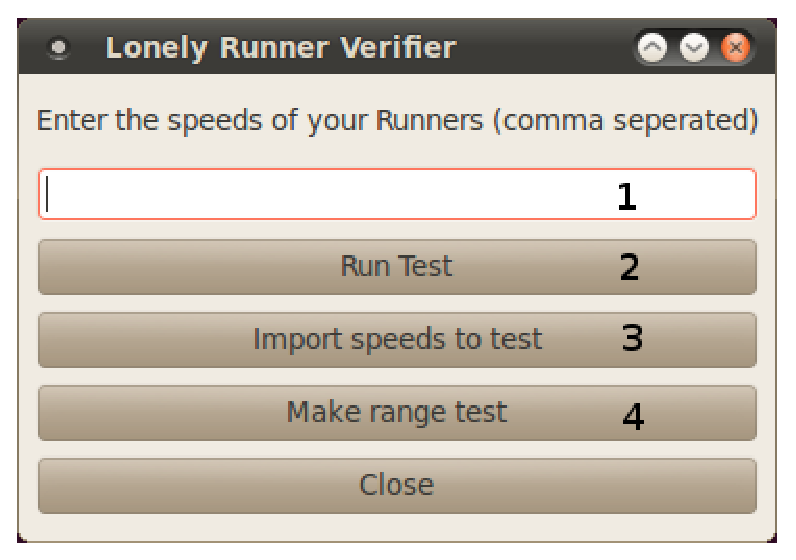
\includegraphics[width=0.45\textwidth]{./images/Lonely_Runner_Verifier}
  \caption{\label{fig:main_window}The main window of the program}
\end{figure}

The labels in figure \ref{fig:main_window} define the following:
\begin{enumerate}
\item The text field to manually enter runner speeds. The speeds must be in $\N$, and should be comma separated.
\item Run the test with the speeds entered in 1. Opens the option pane seen in figure \ref{fig:options}
\item Import the speeds from a JSON file (containing an array of integers). Opens the option pane seen in figure \ref{fig:options}
\item Test a range of configurations. Opens the option pane seen in figure \ref{fig:range_options}
\end{enumerate}

\begin{figure}[H]
  \centering
  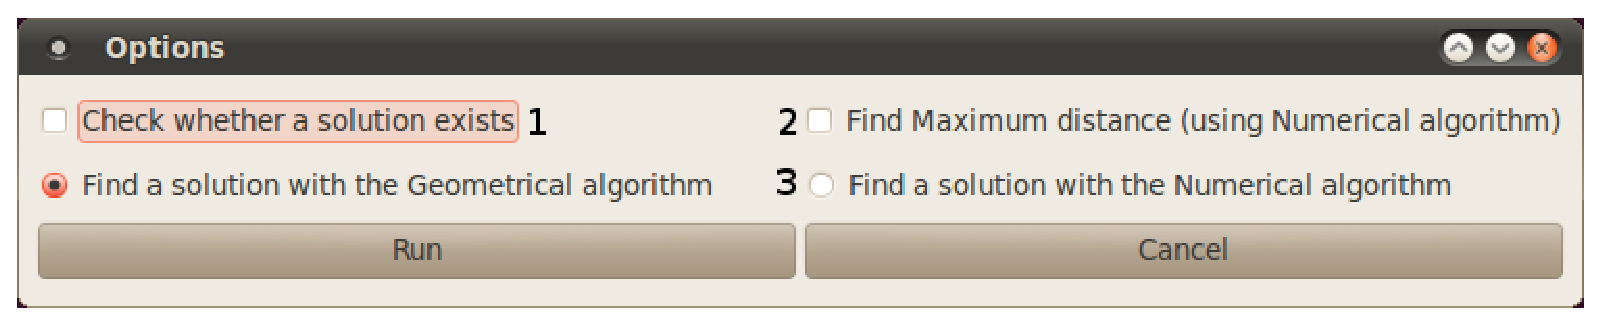
\includegraphics[width=0.70\textwidth]{./images/Options}
  \caption{\label{fig:options}The options for running a single configuration of runners. Accessed by either manually entering a speed or importing a runner configuration}
\end{figure}

The labels in figure \ref{fig:options} define the following:
\begin{enumerate}
\item If checked, the program will perform the check described in Section \ref{detect} before trying the algorithm selected in 3. This option is currently not compatible with option 2.
\item If checked, the program will find and report the maximum value that makes equation \eqaref{eqa:lonelyRunner} hold for the Numerical algorithm. Since this requires an exhaustive search, this can take a while\footnote{Since we in Section \ref{proof_num} established that the worst case run-time for the Numerical algorithm is $O(k * n^3)$, where $k$ is the sum of the 2 largest speeds, and $n$ is the number of Runners.} This option is not currently compatible with option 1.
\item Here you can define whether you would like the configuration to be checked with the Geometrical or the Numerical algorithm.
\end{enumerate}

\begin{figure}[H]
  \centering
  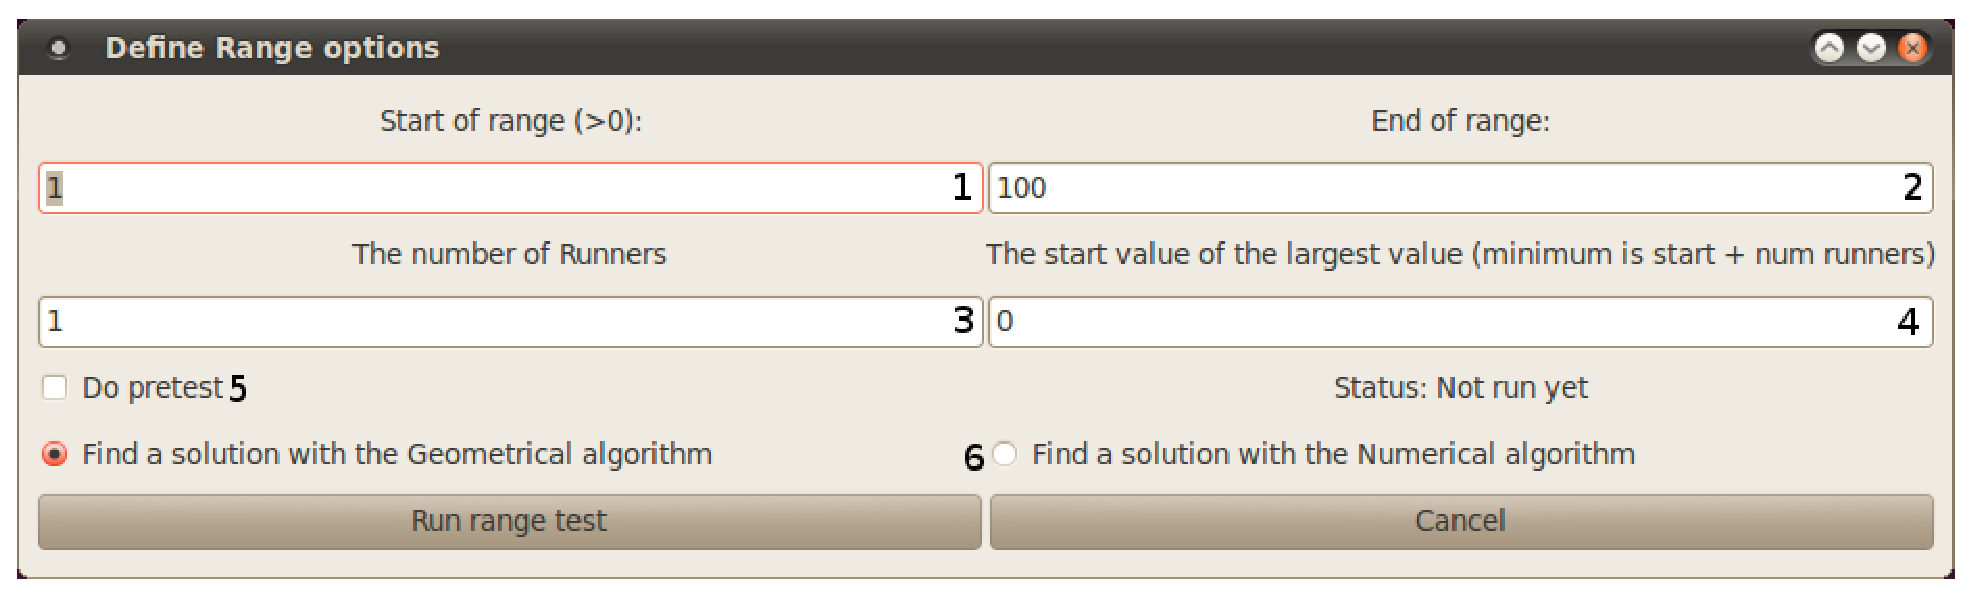
\includegraphics[width=0.70\textwidth]{./images/Range_Options}
  \caption{\label{fig:range_options}The options for running the Range Test}
\end{figure}

The labels in figure \ref{fig:range_options} define the following:
\begin{enumerate}
\item The minimum speed any runner can have 
\item The maximum speed any runner can have
\item The number of runners we are we are going to check
\item The start value of the largest speed. This option can be used as a primitive way to run the task in parallel on multiple computers, or can be used to resume the task at a certain speed. Let $d$ be the minimum speed plus the number of runners minus 1. If the value entered is less than $d$, then $d$ will be used instead.
\item The same as option 1 in figure \ref{fig:options}
\item The same as option 3 in figure \ref{fig:options}
\end{enumerate}

To give an example of the range test, let us say we wanted to test the range 1-10 with 3 runners.

Then the program would create and run the every possible configuration\footnote{This is done without regard to the order of the speeds, as it is clear this does not change the set of valid solutions to equation \eqaref{eqa:lonelyRunner}}, in this order:
$[1, 2, 3], [1, 2, 4], [1, 3, 4], [2, 3, 4], [1, 2, 5], \ldots, [1, 2, 10], \ldots, [7 ,9 ,10], [8, 9, 10]$.

If we still wanted to check the range 1-10 with 3 runners, but set the start value to 9, then the program would create and test the following combinations: 
$[1, 2, 9], [1, 3, 9], [2, 3, 9], \ldots, [7, 8, 9], [1, 2, 10], \ldots, [8, 9, 10]$

It should be clear from the examples above, that even for rather small numbers, a lot of test will be performed, so patience is advised. Since there are only a finite number of combinations, and every combination is either tested by the Geometrical or Numerical algorithm, both of which I have proved to terminate, then the Range Test must terminate.  

\section{Test Results}
\label{test}
\todo{make tests and describe them}

\subsection{Introduction}
In this section I will introduce how I am going to test the algorithms, which parameters I am going to test them on, which software and hardware setup I have tested them on, description of the test themselves, and finally the results.

\subsection{How to test the Algorithms}
Since a configuration of the Lonely Runner conjecture requires $n$ runners and each runner needs a distinct speed, it is clear that the parameters we must test the algorithms for are the number of runners, and their speed. Since the speeds have to be different, I will use the maximum speed to be the defining factor.

To do this test in practice I have choosen to do it in increments, with the number of runners being the deciding factor. If we have to test for $n$ runners, then we let the first configuration to test contain the first $n$ numbers, the second contain from ($n+1$)'th number to the ($2n+1$)'th number and so on.

For example if we have to test 10 runners for values up to 100 with sequential numbers, then the first array to be tested will be [2, 3, 4, $\ldots$, 9, 10, 11], the second array to be tested [12, 13, 14, $\ldots$, 19, 20, 21] and so on.

Since the Lonely Runner conjecture is about the relation between numbers, it would be interesting to test the algorithms in the cases where the numbers are pairwise prime. To do this I have simply calculated the prime numbers up to the maximum value, and used them as the speed.

As a stress test I have also tried calculating the sequential numbers for the 

\subsection{Hardware and software setup}
As mentioned in the implementation part I have implemented the software in C++ using g++ 4.4.3 compiler for Ubuntu. The test was run on a [] \todo{name computer type, hardware, os and so forth once final tests have been made}.

\subsection{Test made} 

I will test both alorithms with 10, 50, 100, 500, 1000 and 2000 runners with a max speed up to 5000 - both for sequential,and prime number speed. For a given configuration the number runners will of course be their minimum speed

\section{Results}
\label{results}
\todo{make results}
In this section I will show and discuss the most important results I have generated by testing the Geometrical and Numerical algorithm against various data-sets detailed in the last section: Prime Numbers, Sequential Numbers and Randomly generated numbers. 

For brevity's sake I have only included the most important graphs, as well as a table detailing the spread and speed of the 2 different algorithms. The complete data-sets can be found in table form in \ref{data_tables}, and is available in the projects github repository.

\subsection{Graphs}

\subsubsection{Primes}
\graph{Primes}{10}{Geo}{Even for small values its clear that the Geometrical algorithm is slower, and that there can be big differences when it runs}
\graph{Primes}{1000}{Geo}{Runners are still slower, but it is also clear that the Numerical algorithm sometimes can use a long time and have quite a spread}

\subsubsection{Sequential numbers}
\graph{Sequential}{10}{Geo}{Even for a small number of runners the Geometrical algorithm can have a very large spread}

\subsubsection{Sequential-Random}
\graph{Sequential-Random}{10}{Geo}{For small randomized values it is clear the Geometrical algorithm is slower than the Numerical algorithm. It is clear that if we remove the exceptional cases from both the Geometrical and Numerical algorithm, then the Geometrical algorithm has the largest spread}
\graph{Sequential-Random}{50}{Geo}{Again it is clear that barring the Numerical instance at index 2600, the Numerical instance is faster than the Geometrical algorithm}
\graph{Sequential-Random}{100}{Geo}{Same as the figure before, but while the Geometrical algorithm is slower compared to \ref{Sequential-Random_50_Geo}, the Numerical algorithm is almost the same}
\graph{Sequential-Random}{1000}{Geo}{Again we see that the Geometrical algorithm is both slower than the Numerical algorithm, and has the largest spread}
\graph{Sequential-Random}{1000}{Num}{}

\hide{
\subsubsection{Random}
\graph{Random}{10}{Num}{}
\graph{Random}{1000}{Geo}{}
\graph{Random}{2000}{Geo}{Again we see that the Numerical algorithm is faster than the Geometrical algorithm}
}
\subsection{Speed}
\input{./data/tables/speed_table.tex}
It is clear from these graphs that the Numerical algorithm is faster for most of the instances. 
I believe the reason for this to belong to the fundamental differences of the 2 algorithms. While both algorithms are based on exploring all possible candidates times for a time where \eqaref{eqa:lonelyRunner} is true, the Geometrical algorithm works by sweeping through the entire first round of the final runner\footnote{The runner with speed 1}, while the Numerical algorithm often is less methodical about it, depending on the 2 selected runner speeds, trying time points against \eqaref{eqa:lonelyRunner}. In practice it is clear this is a better approach than the Geometrical algorithm.
 
It however also clear that for some configurations (even when accounting for the spread), finding a time where \eqaref{eqa:lonelyRunner} is true, takes much more time than most of the other configurations for that number of runners. Two good examples of this are \figureref{Primes_1000_Geo} and \figureref{Sequential-Random_1000_Geo}. The best explanation I have been able to come up with for cases like the first is that \eqaref{eqa:lonelyRunner} depends not so much on the size of the numbers, but rather on the on the number of the runners and the interaction of the runners speeds. I believe cases like the second are caused by the input based run-time of the Numerical algorithm - if the order of the runner speeds are in such a way that a good part of list has to be searched through, then the Numerical algorithms run-time of $O(k * n^3)$ (as proved back in Section \ref{proof_num} on page \pageref{proof_num}) begins to show itself.  

\subsection{Spread}
\input{./data/tables/spread_table.tex}



\subsection{Conclusion}

From the above it is clear that the Numerical algorithm is faster than the Geometrical. It is also clear from the graphs that neither of the algorithms are entirely stable, and for some configurations have both a very large execution time spread. As I have not been able to find a pattern for the configurations that have produced some of these abnormalities, I can 


% [Conclusions are very important. Do not expect that the reader remembers everything you told him/her.
% Having stated the definitions, you can now be more specific that  in the introduction]
% * Overview what this work was about.
% * Main results and contributions
% * Comments on importance or
% * Tips for practical use [how your results or experience can help someone in practice or
%     another researcher to use your simulator or avoid pitfalls]
% * Future work. Reinforce the importance of work, but avoid giving out your ideas].

\section{Conclusion}
\label{conclusion}

\subsection{Summery}

I have in this project:
\begin{itemize}
\item Implemented and tested the Numerical method found in \cite{invis}
\item 
\end{itemize}

\subsection{Results}


\subsection{Future work}

It would be interesting to see whether the Geometrical algorithm could be made faster. One way could be only investigate the intervals where the slowest runner is in the Zone. This is based on the fact that we only have a valid solution if all the runners are in the Zone, which more specifically requires the slowest runner to be in the Zone. This could quite possibly dramatically reduce the required run-time, as since all creations, insertions and removals of Event Points when the runner is outside the Zone would never be made. While the modular nature of the Lonely Runner conjecture might make this seem like a futile task, it is important to remember that it is possible calculate the times where a runner enters the zone, and thus 

Let SlowZone be the interval where the slowest runner is in the zone, then a pair of Event Points should be inserted on the heap iff at least one of \comStart and \comFin is in SlowZone. This would however separate the algorithm into 2 parts: The first part which finds the first Event Points that could be interesting, and the second part which is the same as before, only with a check that does not insert pairs of Event Points that are entirely outside the SlowZone.

\bibliography{LonelyRunner}{}
\bibliographystyle{plain}
\appendix
\section{Spread Tables}
\label{spread_tables}
\subsection{Sequential Results}
\subsubsection{Random Sequential Results}
\begin{table}[bth!]\footnotesize
 \begin{tabular}[3]{c|r|r}
 & Geometrical ($\mu$s) spread & Numerical ($\mu$s) spread\\
\hline
All spreads & 285835 & 1141640236 \\ 
\hline 
Only spreads from calculations & 284813 & 840738 \\ 
that took less than 1 second & & \\ 
\hline
Average spread & 19 & 76190 \\
\hline
Average spread from calculations that & 19 & 56 \\ 
had less spread than 1 second & & \\ 
\end{tabular}\\ \\
\caption{Random Sequential Results\\
The Geometrical algorithm has a lesser spread than the Numerical algorithm by 1141354401 $\mu$s (or 19.0 minutes).\\
The Geometrical algorithm has a lesser spread than the Numerical algorithm by 555925 $\mu$s (or 0.554 seconds), if we disregard every spread that is larger than 1 second.\\
The Geometrical algorithm produced 4 spreads that is larger than 1 second, while the Numerical algorithm produced 7, using 3 data sets (with a total of 14984 data points)\\
}\label{sequential-random_spreadtable}\end{table}

\subsubsection{Non-Random Sequential Results}
\begin{tabular}[3]{c|c|c}
 & Geometrical ($\mu$s) spread & Numerical ($\mu$s) spread\\
\hline
Total spreads & 88221 & 1571476 \\ 
\hline 
Only spreads from runs & 87690 & 41086 \\ 
that took less than 1 second & & \\ 
\hline
Average spread & 5 & 104 \\
\hline
Average spread from runs that & 5 & 2 \\ 
had less spread than 1 second & & \\ 
\end{tabular}\\ \\
The Geometrical algorithm has a lesser spread by 1483255 $\mu$s (or 1.48 seconds) compared to the Numerical algorithm.\\
The Numerical algorithm has a lesser spread by 46604 $\mu$s (or 0.0464 seconds), if we disregard every spread that is larger than 1 second, compared to the Geometrical algorithm.\\
The Geometrical algorithm produced 15 spreads that is larger than 1 second, while the Numerical algorithm produced 15, out of 3 data sets (with a total of 14984 data points)\\


\subsubsection{Combined Sequential Results}
\begin{table}[bth!]\footnotesize
 \begin{tabular}[3]{c|r|r}
 & Geometrical ($\mu$s) spread & Numerical ($\mu$s) spread\\
\hline
All spreads & 374056 & 1143211712 \\ 
\hline 
Only spreads from calculations & 372503 & 881824 \\ 
that took less than 1 second & & \\ 
\hline
Average spread & 12 & 38147 \\
\hline
Average spread from calculations that & 12 & 29 \\ 
had less spread than 1 second & & \\ 
\end{tabular}\\ \\
\caption{Complete Sequential Results\\
The Geometrical algorithm has a lesser spread than the Numerical algorithm by 1142837656 $\mu$s (or 19.0 minutes).\\
The Geometrical algorithm has a lesser spread than the Numerical algorithm by 509321 $\mu$s (or 0.508 seconds), if we disregard every spread that is larger than 1 second.\\
The Geometrical algorithm produced 19 spreads that is larger than 1 second, while the Numerical algorithm produced 22, using 6 data sets (with a total of 29968 data points)\\
}\label{sequential_spreadtable}\end{table}

\subsection{Random results}
\label{random_results}
\subsubsection{Non-sorted Random Results}
\begin{tabular}[3]{c|c|c}
 & Geometrical ($\mu$s) spread & Numerical ($\mu$s) spread\\
\hline
Total spreads & 1748386012 & 4320649261 \\ 
\hline 
Only spreads from runs & 904878576 & 167413192 \\ 
that took less than 1 second & & \\ 
\hline
Average spread & 70148 & 173352 \\
\hline
Average spread from runs that & 36786 & 6729 \\ 
had less spread than 1 second & & \\ 
\end{tabular}\\ \\
The Geometrical algorithm has a lesser spread by 2572263249 $\mu$s (or 42.9 minutes) compared to the Numerical algorithm.\\
The Numerical algorithm has a lesser spread by 737465384 $\mu$s (or 12.3 minutes), if we disregard every spread that is larger than 1 second, compared to the Geometrical algorithm.\\
The Geometrical algorithm produced 326 spreads that is larger than 1 second, while the Numerical algorithm produced 47, out of 5 data sets (with a total of 24924 data points)\\


\subsubsection{Sorted Random Results}

\subsubsection{Combined Results for the Random Numbers}
\begin{table}[bth!]\footnotesize
 \begin{tabular}[3]{c|r|r}
 & Geometrical ($\mu$s) spread & Numerical ($\mu$s) spread\\
\hline
All spreads & 1751142621 & 4322429849 \\ 
\hline 
Only spreads from calculations & 907618766 & 167636694 \\ 
that took less than 1 second & & \\ 
\hline
Average spread & 35129 & 86712 \\
\hline
Average spread from calculations that & 18347 & 3369 \\ 
had less spread than 1 second & & \\ 
\end{tabular}\\ \\
\caption{Complete  Results\\
The Geometrical algorithm has a lesser spread than the Numerical algorithm by 2571287228 $\mu$s (or 42.8 minutes).\\
The Numerical algorithm has a lesser spread than the Geometrical algorithm by 739982072 $\mu$s (or 12.4 minutes), if we disregard every spread that is larger than 1 second.\\
The Geometrical algorithm produced 381 spreads that is larger than 1 second, while the Numerical algorithm produced 102, using 10 data sets (with a total of 49848 data points)\\
}\label{random_spreadtable}\end{table}

\subsection{Prime Results}
\subsubsection{Random Prime Results}
\begin{tabular}[3]{c|c|c}
 & Geometrical ($\mu$s) spread & Numerical ($\mu$s) spread\\
\hline
Total spreads & 656562 & 30502561 \\ 
\hline 
Only spreads from runs & 656562 & 28009439 \\ 
that took less than 1 second & & \\ 
\hline
Average spread & 97 & 4536 \\
\hline
Average spread from runs that & 97 & 4166 \\ 
had less spread than 1 second & & \\ 
\end{tabular}\\ \\
The Geometrical algorithm has a lesser spread by 29845999 $\mu$s (or 29.8 seconds) compared to the Numerical algorithm.\\
The Geometrical algorithm has a lesser spread by 27352877 $\mu$s (or 27.4 seconds), if we disregard every spread that is larger than 1 second, compared to the Numerical algorithm.\\
The Numerical algorithm produced 1 spread that is larger than 1 second out of 10 data sets (with a total of 6724 data points)\\


\subsubsection{Non-Random Prime Results}
\begin{table}[bth!]\footnotesize
 \begin{tabular}[3]{c|r|r}
 & Geometrical ($\mu$s) spread & Numerical ($\mu$s) spread\\
\hline
All spreads & 1716535 & 1658761 \\ 
\hline 
Only spreads from calculations & 1696751 & 1137956 \\ 
that took less than 1 second & & \\ 
\hline
Average spread & 255 & 246 \\
\hline
Average spread from calculations that & 252 & 169 \\ 
had less spread than 1 second & & \\ 
\end{tabular}\\ \\
\caption{Sorted Prime Results\\
The Numerical algorithm has a lesser spread than the Geometrical algorithm by 57774 $\mu$s (or 0.0576 seconds).\\
The Numerical algorithm has a lesser spread than the Geometrical algorithm by 558795 $\mu$s (or 0.558 seconds), if we disregard every spread that is larger than 1 second.\\
The Geometrical algorithm produced 3 spreads that is larger than 1 second, while the Numerical algorithm produced 3, using 10 data sets (with a total of 6724 data points)\\
}\label{prime-normal_spreadtable}\end{table}

\subsubsection{Combined Results for the Primes Numbers} 
\begin{tabular}[3]{c|c|c}
 & Geometrical ($\mu$s) spread & Numerical ($\mu$s) spread\\
\hline
Total spreads & 2373097 & 32161322 \\ 
\hline 
Only spreads from runs & 2353313 & 29147395 \\ 
that took less than 1 second & & \\ 
\hline
Average spread & 176 & 2391 \\
\hline
Average spread from runs that & 175 & 2168 \\ 
had less spread than 1 second & & \\ 
\end{tabular}\\ \\
The Geometrical algorithm has a lesser spread by 29788225 $\mu$s (or 29.8 seconds) compared to the Numerical algorithm.\\
The Geometrical algorithm has a lesser spread by 26794082 $\mu$s (or 26.8 seconds), if we disregard every spread that is larger than 1 second, compared to the Numerical algorithm.\\
The Geometrical algorithm produced 3 spreads that is larger than 1 second, while the Numerical algorithm produced 4, out of 20 data sets (with a total of 13448 data points)\\



\subsection{Total Results}
\subsubsection{Random Total Results}
\begin{tabular}[3]{c|c|c}
 & Geometrical ($\mu$s) spread & Numerical ($\mu$s) spread\\
\hline
Total spreads & 1749581041 & 6658464713 \\ 
\hline 
Only spreads from runs & 906071908 & 196306070 \\ 
that took less than 1 second & & \\ 
\hline
Average spread & 33898 & 129010 \\
\hline
Average spread from runs that & 17672 & 3808 \\ 
had less spread than 1 second & & \\ 
\end{tabular}\\ \\
The Geometrical algorithm has a lesser spread by 4908883672 $\mu$s (or 1.36 hours) compared to the Numerical algorithm.\\
The Numerical algorithm has a lesser spread by 709765838 $\mu$s (or 11.8 minutes), if we disregard every spread that is larger than 1 second, compared to the Geometrical algorithm.\\
The Geometrical algorithm produced 343 spreads that is larger than 1 second, while the Numerical algorithm produced 69, out of 19 data sets (with a total of 51612 data points)\\


\subsubsection{Non-Random Total Results}
\begin{tabular}[3]{c|c|c}
 & Geometrical ($\mu$s) spread & Numerical ($\mu$s) spread\\
\hline
Total spreads & 1804756 & 3230237 \\ 
\hline 
Only spreads from runs & 1784441 & 1179042 \\ 
that took less than 1 second & & \\ 
\hline
Average spread & 83 & 148 \\
\hline
Average spread from runs that & 82 & 54 \\ 
had less spread than 1 second & & \\ 
\end{tabular}\\ \\
The Geometrical algorithm has a lesser spread by 1425481 $\mu$s (or 1.43 seconds) compared to the Numerical algorithm.\\
The Numerical algorithm has a lesser spread by 605399 $\mu$s (or 0.606 seconds), if we disregard every spread that is larger than 1 second, compared to the Geometrical algorithm.\\
The Geometrical algorithm produced 18 spreads that is larger than 1 second, while the Numerical algorithm produced 18, out of 13 data sets (with a total of 21708 data points)\\


\subsubsection{Combined Total Results}
\begin{table}[bth!]\footnotesize
 \begin{tabular}[3]{c|r|r}
 & Geometrical ($\mu$s) spread & Numerical ($\mu$s) spread\\
\hline
All spreads & 1753889774 & 5497802883 \\ 
\hline 
Only spreads from calculations & 910344582 & 197665913 \\ 
that took less than 1 second & & \\ 
\hline
Average spread & 18805 & 58948 \\
\hline
Average spread from calculations that & 9803 & 2122 \\ 
had less spread than 1 second & & \\ 
\end{tabular}\\ \\
\caption{Complete  Results\\
The Geometrical algorithm has a lesser spread than the Numerical algorithm by 3743913109 $\mu$s (or 1.04 hours).\\
The Numerical algorithm has a lesser spread than the Geometrical algorithm by 712678669 $\mu$s (or 11.9 minutes), if we disregard every spread that is larger than 1 second.\\
The Geometrical algorithm produced 403 spreads that is larger than 1 second, while the Numerical algorithm produced 128, using 36 data sets (with a total of 93264 data points)\\
}\label{total_spreadtable}\end{table}



\end{document}
